\chapter{PCB
\index{Chapter!PCB}
\index{PCB}
\label{PCB}}
\section{Schematic}
\subsection{ORCad Capture Overview}
ORCad comes with a schematic software called Capture CIS which we used to create our schematics. As a reference to both us and others, this section is
dedicated to providing a small walkthrough to using the software and some nice-to-know features.
\begin{figure}[H]
  \centering
  \scalebox{.3}{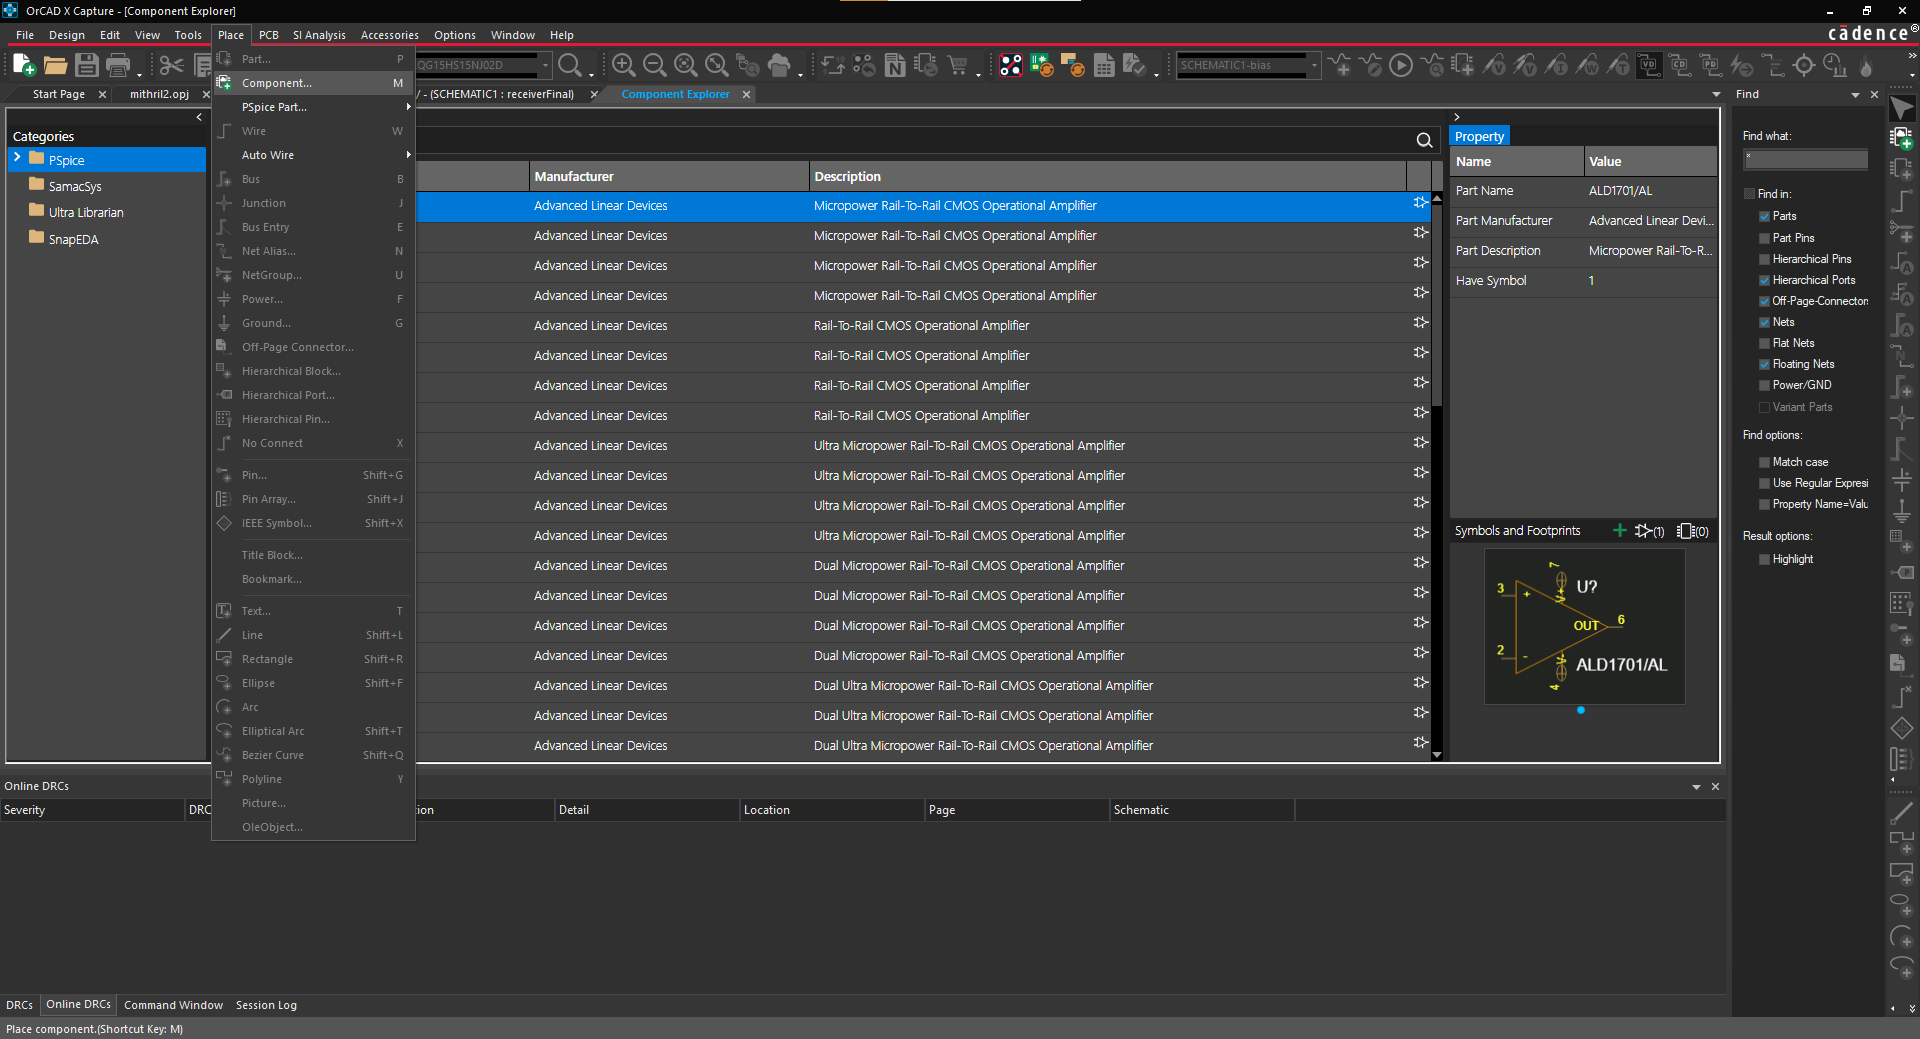
\includegraphics{CaptureImages/ultralib.png}}
\caption{Component Database Search}
\label{img:ultralib}
\end{figure}

The first important feature we found was the component database, which can be seen in Figure \ref{img:ultralib}. By clicking on the icon that has a small chip and cloud will 
take you to this page which contains subdirectories "PSpice" "SamacSys" "UltraLibrarian" and "SnapEDA". PSpice contains parts that
have simulation properties, but we ignored this as we did not know how to use PSpice. The other three are different databases
containing schematic symbols and layout footprints for parts that can be found on major retailers like DigiKey, Mouser, and Arrow.

\begin{figure}[H]
  \centering
  \scalebox{.5}{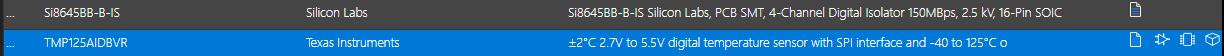
\includegraphics{CaptureImages/ultralibexample.png}}
\caption{Schematic/Footprint Examples}
\label{img:ultralibexample}
\end{figure}

You can search for parts in the search fields for the different databases to try to find a part that has a schematic symbol
and footprint available. You can see in Figure \ref{img:ultralibexample} that parts with the symbol and footprint available will
have an amp and chip symbol next to them. The box means there is a 3D CAD model associated with them too. If you cannot find
the symbol and footprint for a part, we recommend going on Mouser and finding the part, then requesting the symbol and footprint.
Usually, the schematic and footprint will be added to SamacSys after a couple of days.

\begin{figure}[H]
  \centering
  \scalebox{.3}{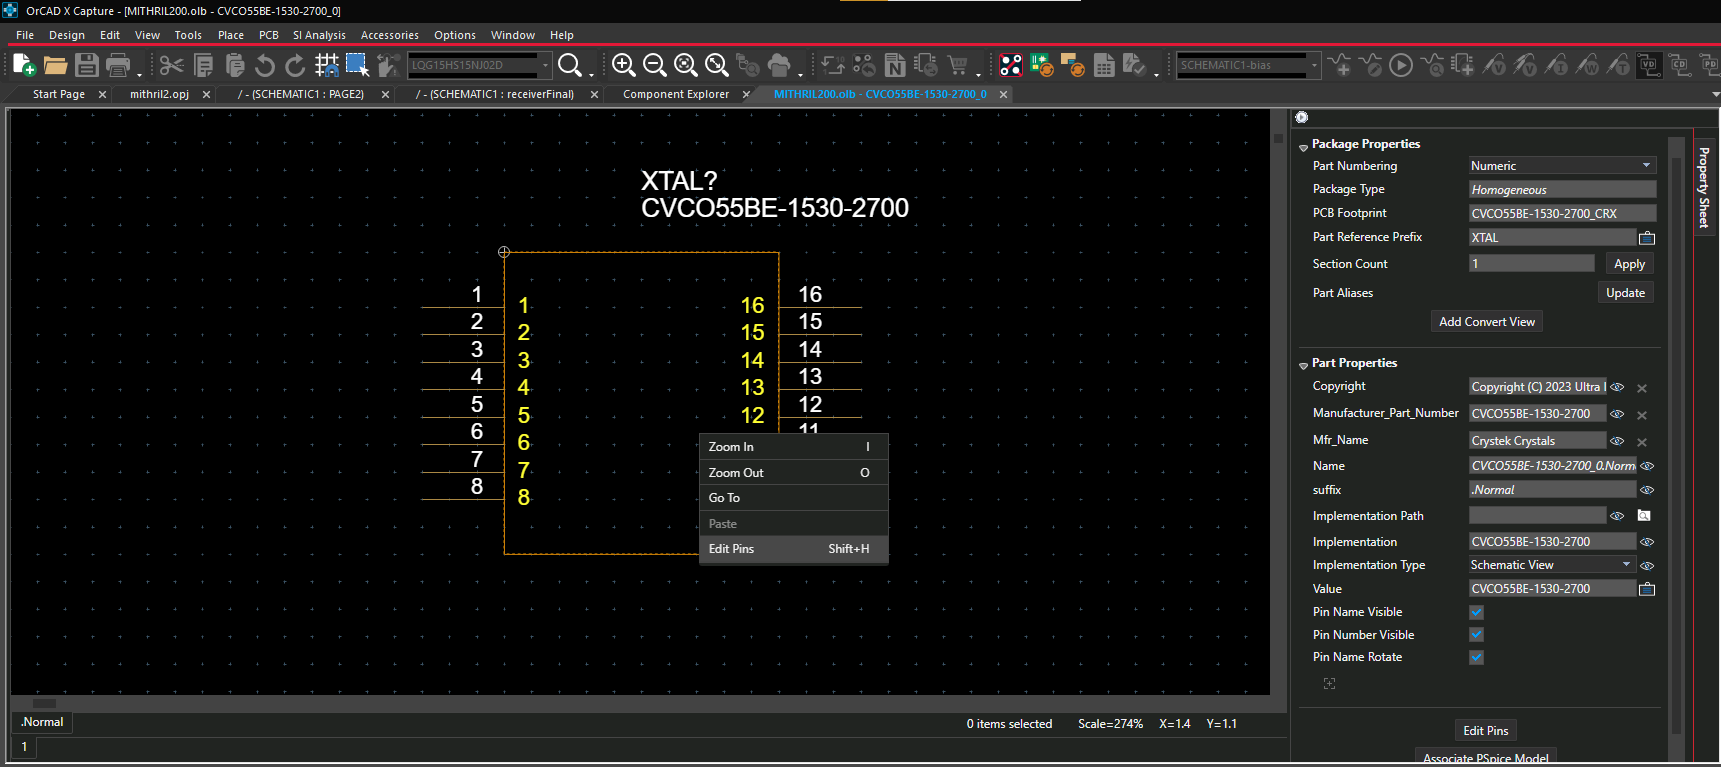
\includegraphics{CaptureImages/editpin.png}}
\caption{Editing Schematic Parts}
\label{img:editpart}
\end{figure}

Sometimes, these symbols and footprints are not correct. If the schematic symbol is incorrectly labeled, you can edit the part,
then click edit pins to make sure all the pins are correctly labeled and numbered as can be seen in Figure \ref{img:editpart}.

\begin{figure}[H]
  \centering
  \scalebox{.3}{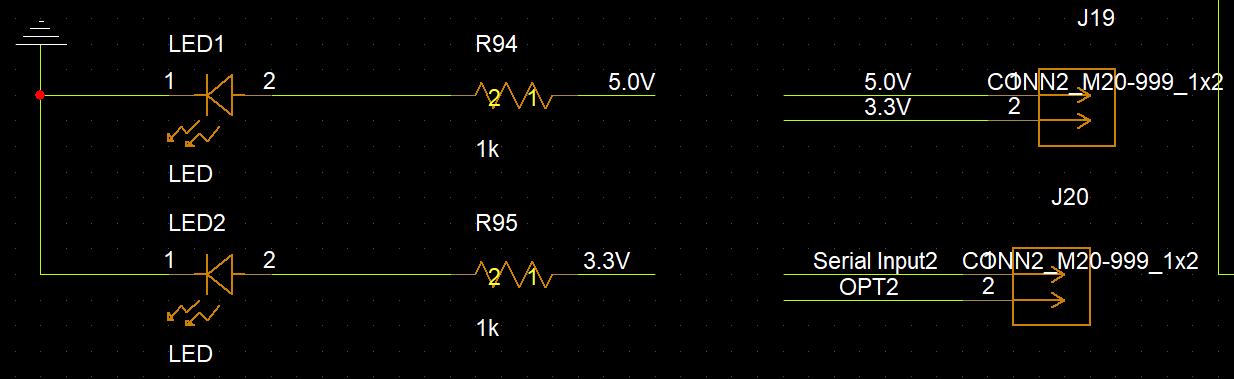
\includegraphics{CaptureImages/wirealias.png}}
\caption{Wires and Net Alias}
\label{img:wirealias}
\end{figure}

Once you've placed your parts down in the schematic, now comes time to connect everything together. To navigate through the
schematic interface, you can use CTRL+Scroll Wheel to zoom in and out, and middle mouse button to scroll left to right.

You can use "w" to enter wiring mode, which lets you place down wires according to your grid size. After wiring, be sure to use
"n" to enter net alias mode and assign aliases to your wires. As can be seen in Figure \ref{img:wirealias}, there are two
non-connected wires both with the alias "5.0V". This effectively connects them since they are under the same alias and will also
label them in the layout when routing. Using the net alias helps with things like power where connecting everything that needs
power with a wire to your power source would make the schematic a mess. In short, all wires with the same net alias are considered
connected.

\begin{figure}[H]
  \centering
  \scalebox{.3}{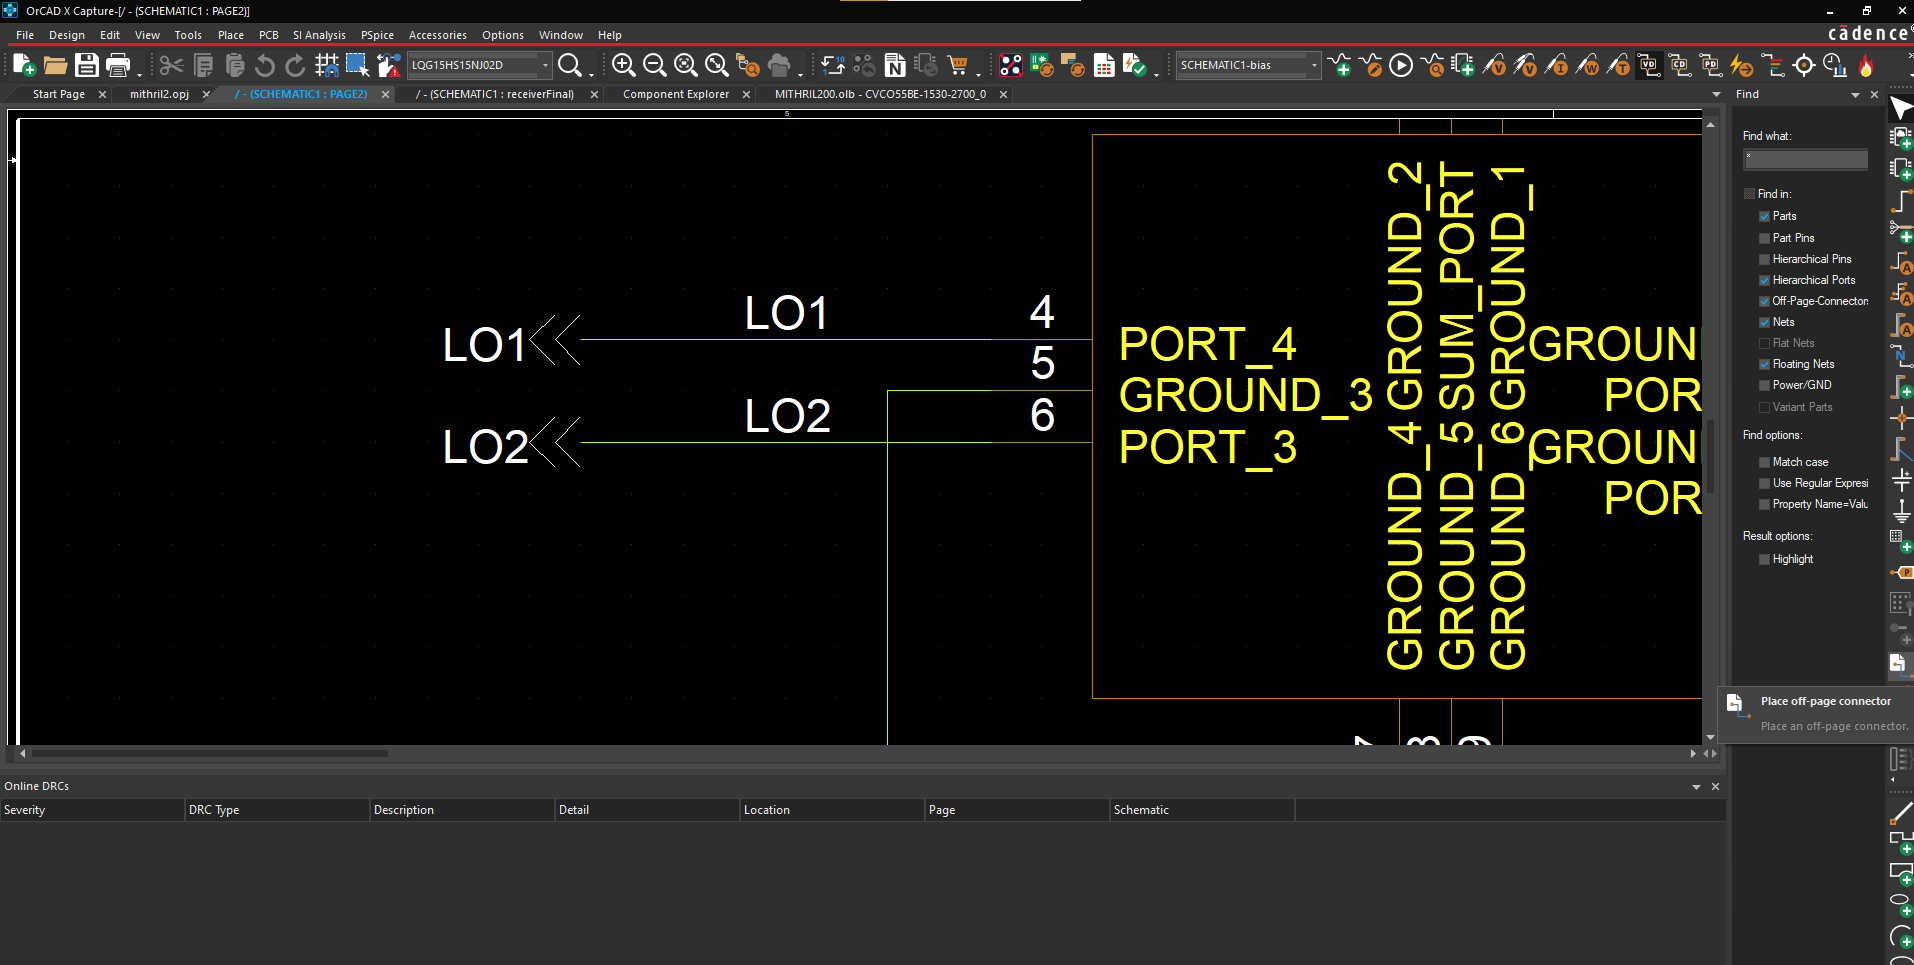
\includegraphics{CaptureImages/offpageconn.png}}
\caption{Off Page Connectors}
\label{img:offpageconn}
\end{figure}

If you run out of room or want to separate your schematics into different pages, you can connect wires from different schematic
pages using off-page connectors as shown in Figure \ref{img:offpageconn}. Connect the off-page connector to a wire and name it
the same on both schematic pages to have the wires connect.

\subsection{Circuitry Good Practices}
\subsubsection{DC Blocking and Coupling Caps}
\begin{figure}[H]
  \begin{minipage}{0.5\textwidth}
    \centering
    \scalebox{.3}{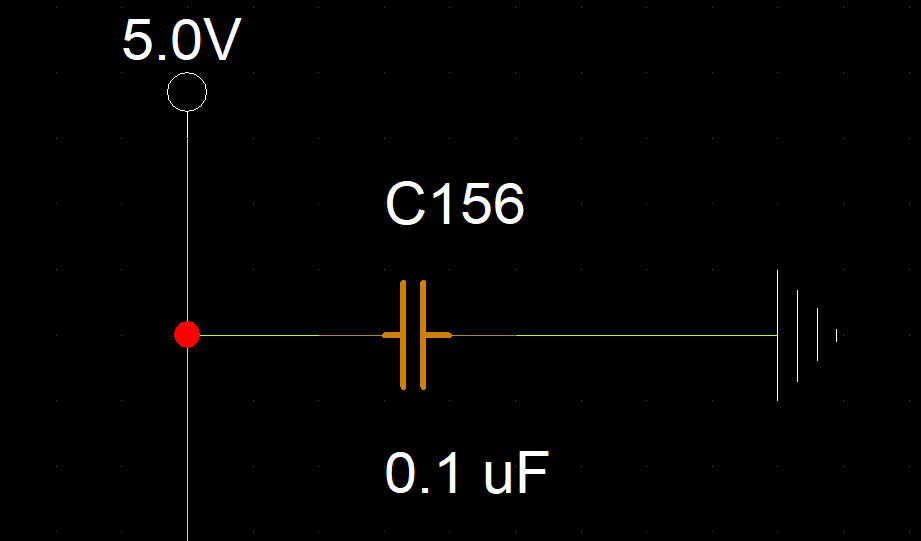
\includegraphics{CaptureImages/coupling.png}}
    \caption{Coupling Capacitor}
    \label{img:couplingcap}
  \end{minipage}
  \begin{minipage}{0.5\textwidth}
    \centering
    \scalebox{.3}{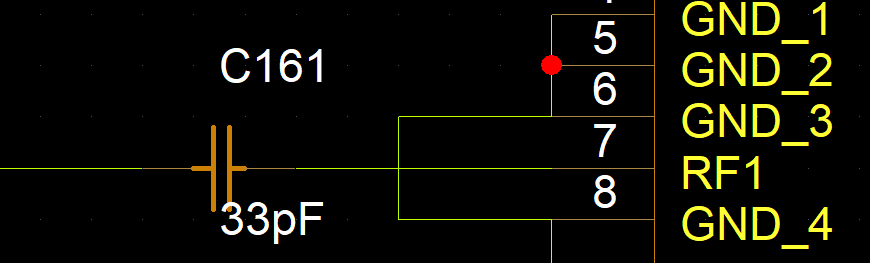
\includegraphics{CaptureImages/dcblocking.png}}
    \caption{DC Blocking Capacitor}
    \label{img:dcblockingcap}
  \end{minipage}
\end{figure}

Two good practices to include in your schematics are coupling and DC blocking capacitors. 

Coupling capacitors are usually used when giving power to some component or chip as can be seen in Figure \ref{img:couplingcap}. It 
can be thought of as a mini low-pass filter, where the capacitance of your coupling capacitor will affect the 
cutoff frequency of the filter. These coupling capacitors should be placed in parallel with the power wire that goes into the chip.

DC Blocking capacitors do the exact opposite, and are usually used when passing a signal from one component to another as can be 
seen in Figure \ref{img:dcblockingcap}. They can be thought of as mini high-pass filters, where the capacitance of the DC Blocking
capacitor affects the cutoff frequency. These are placed in series with the signal wire.
\begin{figure}[H]
\begin{equation}
  C = \frac{1}{2\pi Xf}
  \end{equation}
  \caption{Capacitance of a Coupling or DC Blocking Capacitor}
  \label{eq:capacitance}
\end{figure}
The equation for finding the capacitance of either the coupling or DC blocking capacitor can be seen in Equation \ref{eq:capacitance} 
where C is the capacitance, X is the impedance, and f is the cutoff frequency.
Essentially, a higher cutoff frequency corresponds to a lower capacitance value, and the only difference between the coupling and
DC blocking capacitor is the coupling capacitor passes everything below that cutoff frequency, and the DC blocking capacitor passes
everything above that cutoff frequency.
\subsubsection{Test Pins and Grounds}
\begin{figure}[H]
  \centering
  \scalebox{.3}{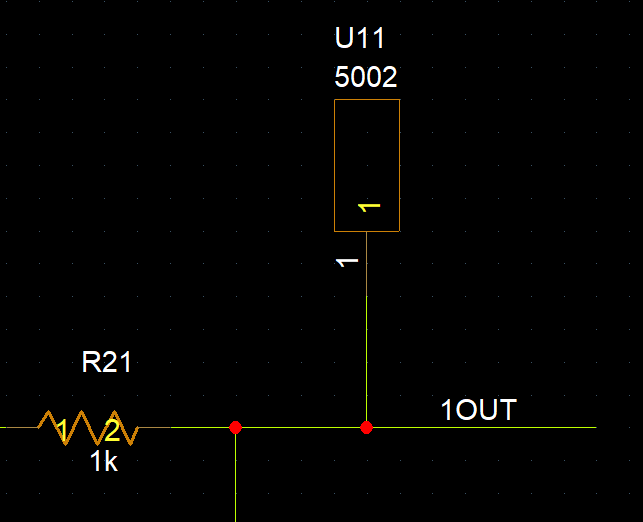
\includegraphics{CaptureImages/testpin.png}}
\caption{Test Pin}
\label{img:testpin}
\end{figure}

Other extremely important things to add are test pins as seen in Figure \ref{img:testpin} and exposures to ground. Credit to
Professor Muresan for telling us to add both of these as they were vital to testing and the operation of the board.

Test pins should be placed in parallel with signal wires so that you can hook in with an oscilloscope and examine what is happening.
Really, after every stage in a signal chain it would be good practice to expose the signal via a test pin or if it is RF with an
SMA connector. This allows you to debug analog things and find out how each stage is affecting your signal. We only added it
in one place and after the fact wished we had placed more test pins so we could see what was happening from component to component.

Ground pins and pads are also really important. We overlooked adding a ground pin which was extremely inconvenient for us, and wished we
had put ample ground pins and pads everywhere on the board. These are necessary if using external components with the board, since
they should have a common ground.

\subsubsection{Power LEDs}
\begin{figure}[H]
  \centering
  \scalebox{.3}{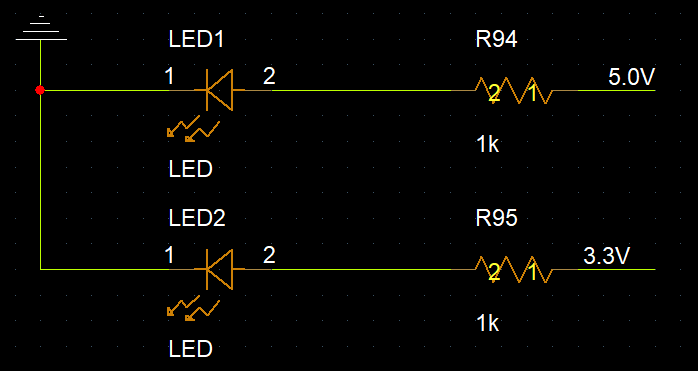
\includegraphics{CaptureImages/leds.png}}
\caption{Power LEDs}
\label{img:led}
\end{figure}

Another nice thing to have are some LEDs connected to power, just so you know at the very least your board is turned on and everything
is receiving power. Having a switch of some sort to block power is also something nice to have which we did not add.

\subsubsection{Potentiometers}
\begin{figure}[H]
  \centering
  \scalebox{.3}{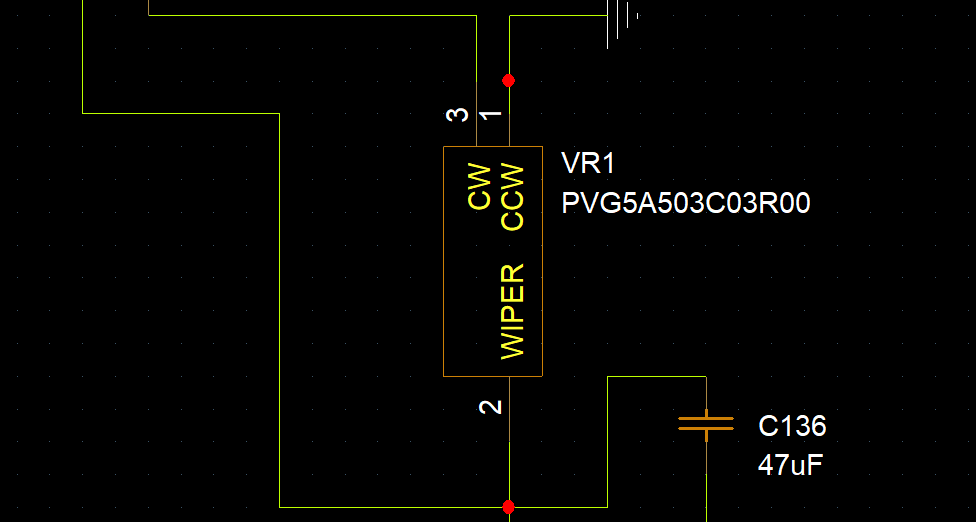
\includegraphics{CaptureImages/pot.png}}
\caption{Potentiometers}
\label{img:pot}
\end{figure}

Another extremely useful thing to add is potentiometers, as can be seen in Figure \ref{img:pot}. In things like amplifying or
filtering stages where resistors can change the cutoff frequency or gain of your circuit, potentiometers are very useful. From
Figure \ref{img:pot}, we can see that potentiometers have three ports: CCW, CW, and Wiper. How potentiometers work is that the
wiper controls the resistance of the potentiometer, and turning it CW will make more signal go in that port, and turning it CCW will
make more signal go into that port (oversimplified explanation). Therefore, it can be set up by just feeding the input to the wiper,
the output to CCW, and CW to ground. This can help with changing gains and cutoff frequencies even after the board is printed and
assembled.

\subsection{Transmitter}
\subsection{Receiver}

\section{Layout}
\